\documentclass[article]{jlreq}

\usepackage{tcolorbox}      %
\usepackage{url}            % URL
\usepackage{pxrubrica}      % ルビ
\usepackage{siunitx}        %
\usepackage{tasks}          %
\usepackage{array}          %
\usepackage{booktabs}       %
\usepackage{amsmath}        %
\usepackage{textcomp}       %
\usepackage{msc}            % シーケンス図
\usepackage{flowchart}      % フローチャート



\title{Lua\LaTeX \\ ---テンプレート---}
\author{Author}
\date{\today}

\begin{abstract}
アブストラクトを書くところ
\end{abstract}

\begin{document}
\maketitle
\setcounter{tocdepth}{2}
\tableofcontents
\newpage

\section{〜〜とは}
本章では、、、

\subsection{〜〜の成り立ち}
本節では、、、

\subsubsection{〜〜の発生}
本項では、、、

\begin{quote}
	あのイーハトーヴォのすきとおった風、夏でも底に冷たさをもつ青いそら、
	うつくしい森で飾られたモリーオ市、郊外のぎらぎらひかる草の波。
\end{quote}


\section{人間の諸特性}
本章では2、、、

\subsection{身体的特性}
本節では2、、、

\subsubsection{静的形態特性}
本項では2、、、

\begin{table}[h]
\centering
\caption{PTS法(MODAPT法)による動作時間の例}
\label{MODAPT}
\begin{tabular}{cccc}
\toprule
移動時間 [cm] & 身体部位 & 動作時間 [sec] & 比率 \\
\midrule
約2.5 & 指 & 0.129 & 1 \\
約5 & 手首から先 & 0.258 & 2 \\
約15 & 前腕 & 0.387 & 3 \\
\bottomrule
\end{tabular}
\end{table}

箇条書きの例。
\begin{itemize}
\item ユーザの許容範囲の共通範囲を採用する(例:自動販売機)
\item 立場の弱いユーザに合わせる(例:公園の水飲み場)
\end{itemize}

立場の弱いユーザに合わせる場合や,ユーザ層ごとに設計する場合には,
全体として5\textasciitilde95\%ileのユーザを保証しなければならない.
なお,\emph{安全性に関わる部分では1\textasciitilde99\%ileのユーザを保証する必要がある.}

\begin{figure}[h]
\centering
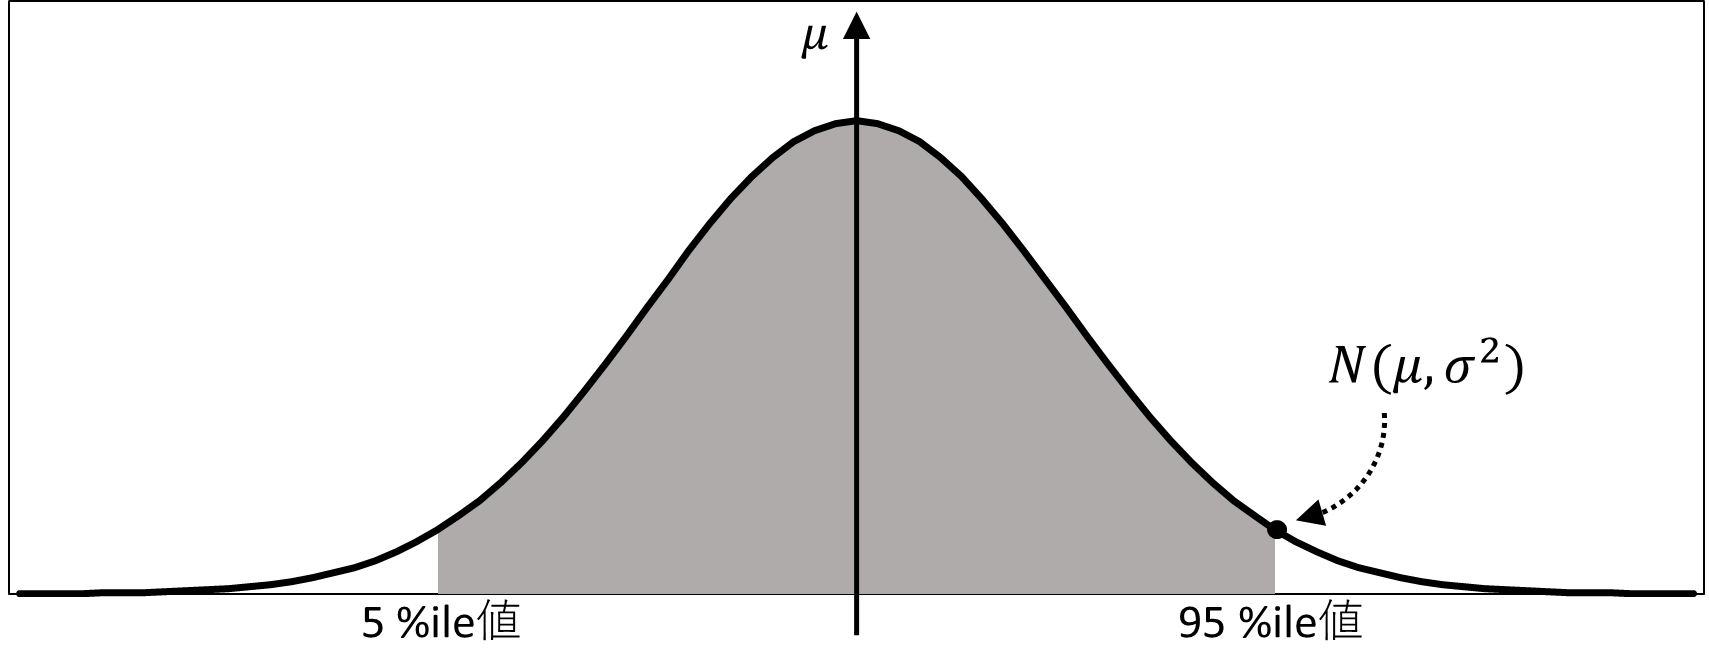
\includegraphics[width=13cm]{img/fig.png}
\caption{パーセンタイル}
\end{figure}


\section{mscを使ったシーケンス図}

\begin{msc}{Example}
    \declinst{usr}{User}{}
    \declinst{m1}{Machine 1}{control}
    \declinst{m2}{Machine 2}{drill}

    \mess[label position=below]{startm1}{usr}{m1}
    \nextlevel
    \mess{startm2}{m1}{m2}
    \nextlevel
    \mess{log}{m1}{envleft}
    \nextlevel
    \nextlevel
    \mess{output}{m2}{usr}[2]
    \mess{free}{m1}{usr}
    \nextlevel
\end{msc}


\begin{msc}{Simple Sequence Diagram}

  % インスタンスの宣言
  \declinst{user}{User}{}
  \declinst{server}{}{Server}

  % メッセージのやり取り
  \mess{Request}{user}{server}  % "Request" というメッセージを user から server へ送信
  \nextlevel
  \nextlevel
  \mess[side=right]{Process}{server}{server}[-1]  % server が自身で "Process" を実行
  \nextlevel
  \mess{Process}{server}{server}[1]  % server が自身で "Process" を実行
  \nextlevel
  \nextlevel
  \mess{Response}{server}{user}  % server から user へ "Response" というメッセージを送信
\end{msc}


\begin{msc}[small values]{Label reference points}
    \declinst{m0}{I0}{}
    \declinst{m1}{I1}{}
    \declinst{m2}{I2}{}
    \nextlevel
    \mess[label position=above]{above}{m0}{m1}
    \nextlevel
    \mess[label position=below]{below}{m1}{m2}
    \nextlevel[2]
    \mess[anchor=south,pos=0.1]{south}{m1}{m0}
    \nextlevel
    \mess[anchor=north]{north}{m2}{m1}
    \nextlevel[2]
    \mess[label position=left]{left}{m0}{m0}[2]
    \mess[side=right,pos=0.9]{right}{m2}{m2}[2]
    \nextlevel[4]
    \mess[label position=right]{right}{m0}{m0}[2]
    \mess[left,side=right]{left}{m2}{m2}[2]
    \nextlevel[6]
    \mess[anchor=east]{east}{m0}{m0}[-2]
    \mess[anchor=west,side=right]{west}{m2}{m2}[-2]
    \nextlevel[4]
    \mess[right]{right}{m0}{m0}[-2]
    \mess[side=right,left]{left}{m2}{m2}[-2]
    \nextlevel[2]
    \mess[below left]{below left}{m0}{m1}[2]
    \mess[above right]{above right}{m1}{m2}[2]
    \nextlevel[6]
    \mess[anchor=south west]{SW}{m1}{m0}[-2]
    \mess[anchor=north east,pos=0]{NE}{m2}{m1}[-2]
    \nextlevel[2]
\end{msc}



\end{document}
